\documentclass{beamer}

\usepackage[utf8]{inputenc}
\usetheme{Madrid}
\title{Garbage bins placing for maximum demand satisfaction}
\author{Indre Bogdan}
\institute{Department of Computer Science\\Technical University of Cluj-Napoca}
\date{2020}
 
\begin{document}
 
\frame{\titlepage}
 
\begin{frame}
\frametitle{\centerline{Genetic Algorithms \& DEAP}}
\begin{enumerate}
\item\pause Distributed Evolutionary Algorithms in Python \pause
\item Evolutionary Framework \pause
\item Fast prototyping and testing of ideas
\end{enumerate}
\end{frame}

\begin{frame}
\frametitle{\centerline{The problem}}
\begin{enumerate}
\item\pause Waste, waste everywhere \pause
\item Expensive
\end{enumerate}
\end{frame}

\begin{frame}
\frametitle{\centerline{The Scenario}}
\begin{enumerate}
\item \pause Demand \pause
\item Distance \pause
\item Budged
\end{enumerate}
\end{frame}

\begin{frame}
\frametitle{\centerline{A solution?}}
\begin{enumerate}
\item \pause Many actually \pause
\item Genetic Algorithms
\end{enumerate}
\end{frame}
 
\begin{frame}
\frametitle{\centerline{A solution}}
\begin{enumerate}
\item Input
\begin{enumerate}
\item \pause Map with historical data \pause
\item Number of bins \pause
\end{enumerate}
\item Output
\begin{enumerate}
\item \pause Map with the location of the bins, also their minimum volume \pause
\item And something else
\end{enumerate}
\end{enumerate}
\end{frame}

\begin{frame}
\begin{figure}[H]
    \centering
    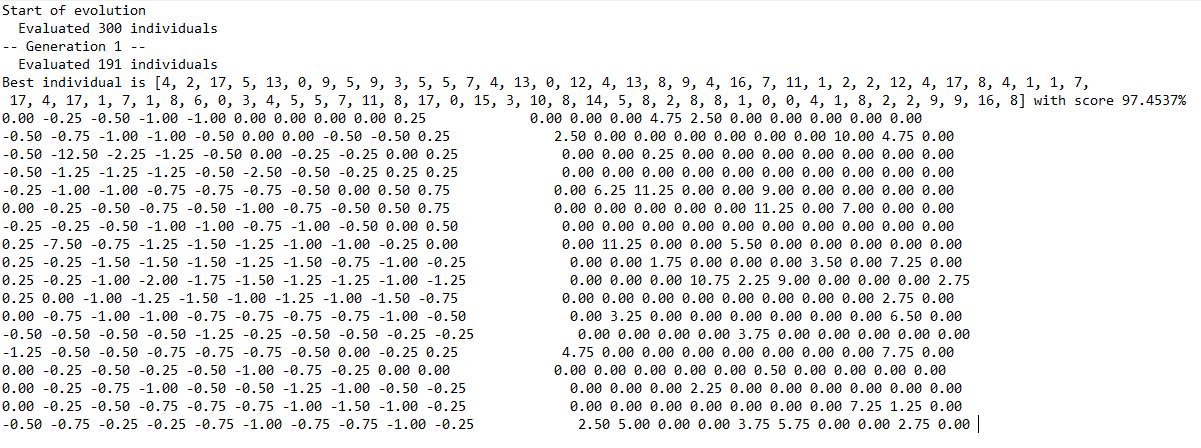
\includegraphics[width=1\textwidth]{fig/results1}
    \caption{An iteration}
    \label{fig:results1}
\end{figure}
\end{frame}

\begin{frame}
\begin{figure}[H]
    \centering
    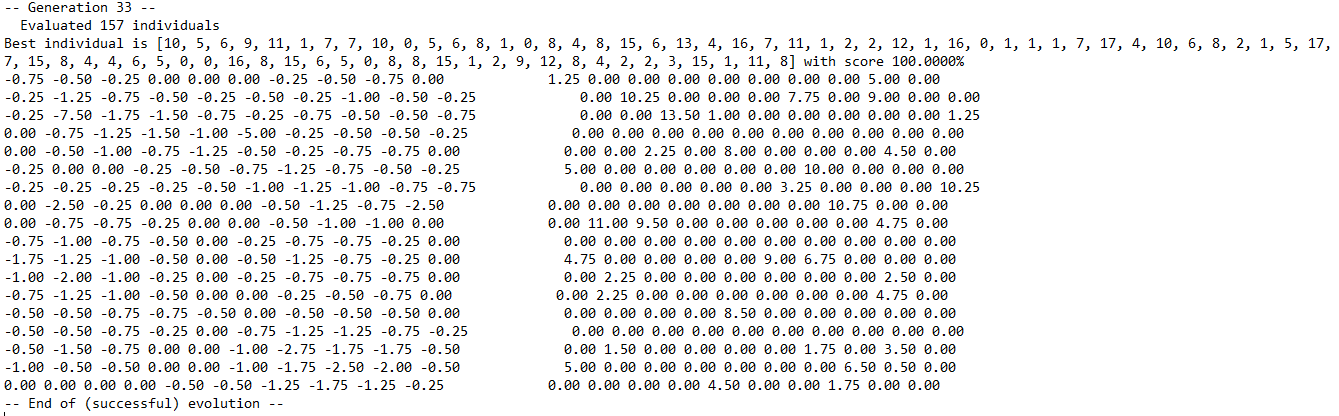
\includegraphics[width=1\textwidth]{fig/results3}
    \caption{A result}
    \label{fig:results3}
\end{figure}
\end{frame}

\begin{frame}
\center {Thank you!}
\end{frame}
\end{document}